\documentclass[t]{beamer}

% Load general definitions
% Preamble file - general definitions, package loading, etc.

%=================================
% Load packages
\usepackage{amssymb,amsmath}
\usepackage{graphicx}
\usepackage{url}
\usepackage{tikz}
\usetikzlibrary{mindmap,trees,arrows}
\usepackage{fancyvrb}
\usepackage[portuguese]{babel} 
\usepackage[utf8]{inputenc}
\usepackage{subfigure}
\usepackage{times}
\usepackage[T1]{fontenc}
\usepackage{cancel}
\usepackage{color}
\usepackage{listings}
\usepackage[document]{ragged2e}
\usepackage{hyperref}
\usepackage{listings}


%=================================
% Set mode
\mode<presentation>
{
	\usetheme{Madrid}
	\usecolortheme{structure}
	\useoutertheme{infolines}
	\setbeamercovered{invisible}
}

% Get rid of nav bar
\beamertemplatenavigationsymbolsempty

% Insert frame number at bottom of the page.
\usefoottemplate{\hfil\tiny{\color{black!90}\insertframenumber}} 

%=================================
% Define new commands

\newcommand\Real{{\mathbb{R}}}
%\newcommand{\vi}{\vspace{0.6\baselineskip}}
%\newcommand{\goodgap}{\hspace{\subfigtopskip}\hspace{\subfigbottomskip}}


% Equation environments
\newcommand{\beq}{\begin{equation}}
\newcommand{\eq}{\end{equation}}
\newcommand{\beqs}{\begin{equation*}}
\newcommand{\eqs}{\end{equation*}}
\newcommand{\beqn}{\begin{eqnarray}}
\newcommand{\eqn}{\end{eqnarray}}
% Bold variables
\newcommand{\mbf}[1]{\ensuremath{\mathbf{#1}}}
% Itemization
\newcommand{\bitem}{\begin{itemize}}
\newcommand{\eitem}{\end{itemize}}
\newcommand{\spitem}{\vskip 1em\item}
\newcommand{\bitems}{\begin{itemize}\item}
\newcommand{\benums}{\begin{enumerate}\item}
\newcommand{\eenum}{\end{enumerate}}
% color blocks
\newenvironment{colorblock}[2]{%
\setbeamercolor{block title}{#2}
\begin{block}{#1}}{\end{block}}
% Vertical spacing
\newcommand{\vone}{\vskip 1em}
\newcommand{\vhalf}{\vskip .5em}
% Frame environments
\newenvironment{ftst}[3][t]{%
\begin{frame}{environment=ftst,#1}
\frametitle{#2}
\framesubtitle{#3}}{\end{frame}}
\newenvironment{ftstf}[2]{
\begin{frame}[fragile,environment=ftstf]
\frametitle{#1}
\framesubtitle{#2}}{\end{frame}}
% colors
\definecolor{MyGray}{rgb}{0.5,0.5,0.5}
\definecolor{MyDBGray}{rgb}{0.1,0.1,0.4}
\definecolor{darkgreen}{rgb}{0,0.4,0}
\definecolor{black}{rgb}{0,0,0}
\def\defn#1{{\color{red} #1}}
% Footnote
\renewcommand{\thefootnote}{\alph{footnote}}
% Relaxed footnotes
\newcommand{\lfr}[1]{\let\thefootnote\relax\footnote{\tiny #1}}
% Verbatim environment - using FANCYVRB package
\DefineVerbatimEnvironment%
{rcode}{Verbatim}
{fontsize=\scriptsize}

% Verbatim environment - using LISTINGS package
%\lstnewenvironment{rcode} {\lstset{	language = R,
%									basicstyle = \scriptsize\ttfamily,
%									showspaces = false,
%									showstringspaces = false,
%									showtabs = false,
%									keywordstyle = \color{black}\bfseries,
%									commentstyle = \color{darkgreen},
%									numbers = none,
%									otherkeywords={	<-,
%													ggplot,
%													geom_boxplot,
%													facet_grid,
%													shapiro.test,
%													fligner.test,
%													glht,
%													with},
%									deletekeywords={data,
%													model,
%													residuals,
%													c,
%													axis,
%													default,
%													labels,
%													qq.text}}}%
%{}

% Specific definitions
\title[]{Tópicos Especiais em Computação I}
\subtitle[]{Análise de Dados}
\author[]{Patrícia Lucas\\{\footnotesize }}
\institute{Bacharelado em Sistemas de Informação \\ IFNMG  - Campus Salinas}
\date{\scriptsize Salinas\\Março 2021}

\begin{document}

% cover page
\setbeamertemplate{footline}{}
\begin{frame}

\begin{center}
\includegraphics[width=.15\textwidth]{}
\end{center}
  \titlepage
  \begin{tikzpicture}[remember picture,overlay]
  \node[anchor=south east,xshift=-5pt,yshift=5pt] at (current page.south east) {\tiny Versão 1.2021};
  \node[anchor=south west,yshift=0pt] at (current page.south west) {
\includegraphics[width=.25\textwidth]{Logos/salinas_horizontal_jpg.jpg}};
  \end{tikzpicture}  
\end{frame}

% Main slides
\begin{ftst}{Referência}{Análise dos dados}

\begin{figure}
    
\includegraphics[scale=0.35]{Figuras/slide01_11.jpg}
\end{figure}
Capítulo 2: Análise de dados.
\vone
\scriptsize
Inteligência Artificial: Uma abordagem de aprendizado de máquina. Katti Faceli...[et al.]. - Rio de Janeiro: LTC, 2011.

\end{ftst}

%=====
%=====

\begin{ftst}{Conjuntos de dados}{Introdução}

Apesar do crescente número de bases de dados disponíveis, na maioria das vezes não é possível utilizar algoritmos de aprendizado de máquina diretamente sobre esses dados.
\vone
A análise dos dados e as técnicas de pré-processamento são frequentemente utilizadas para tornar os conjuntos de dados mais adequados para o uso desses algoritmos.
\vone


\end{ftst}

%=====

\begin{ftst}{Análise dos dados}{Análise dos dados}

A análise das características presentes em um conjunto de dados permite a descoberta de padrões e tendências que podem fornecer informações valiosas que ajudem a compreender o processo que gerou os dados.
\vone
Muitas dessas características podem ser obtidas por meio da aplicação de fórmulas estatísticas simples ou podem ser observadas por meio do uso de técnicas de visualização.

\end{ftst}

\begin{ftst}{Exploração de dados}{Análise dos dados}

Uma grande quantidade de informações úteis pode ser extraída de um conjunto de dados por meio de sua análise ou exploração.
\vone
Informações obtidas durante a exploração podem ajudar na escolha da técnica mais apropriada de pré-processamento e também do aprendizado.
\vone
A estatística descritiva resume de forma quantitativa as principais características de um conjunto de dados como, por exemplo:

- Frequência.

- Localização ou tendências central (ex: média).

- Dispersão ou espalhamento (ex: desvio padrão).

- Distribuição ou formato.


\end{ftst}

%=====

\begin{ftst}{Exploração de dados}{Dados univariados}
\textbf{Dados univariados:} quando o objeto possui apenas um atributo.
\vone
\textit{Medidas de localidade:} definem pontos de referência nos dados.\\
Ex: moda, média, mediana e os quartis.
\vone
\begin{itemize}
    \item Média: dado um conjunto de $n$ valores numéricos $x = {x_1, x_2, ..., x_n}$, o valor médio desse conjunto é dado pela Equação \ref{eq:media}:
    \begin{equation}
        \centering
        \overline{x} = \frac{1}{n} \sum_{i=1}^{n}{x_i}
        \label{eq:media}
    \end{equation}
\end{itemize}
\vone

\end{ftst}

%=====

\begin{ftst}{Exploração de dados}{Dados univariados}
\textbf{OBS: a média é sensível a \textit{outliers}!}
\vone
\textit{Outliers} são valores muito diferentes dos demais valores observados para um mesmo atributo. Vamos verificar isso...
\vone
Uma turma de 7 alunos possui as seguintes idades: \\
\begin{center}
    ${18,19,20,20,23,24,24}$.\\
\end{center}

A média de idades dessa turma é: $21,1$.
\vone
Supondo que um aluno de 80 anos entre para essa turma, a média passaria a ser $28,5$. 
\vone
Dessa forma, percebemos que a média é um bom indicador do meio de um conjunto apenas se os valores estão distribuídos simetricamente.
\end{ftst}

%=====

\begin{ftst}{Exploração de dados}{Dados univariados}
O problema com os \textit{outliers} é minimizado com o uso da mediana.
\vone
\begin{itemize}
    \item Mediana: dado um conjunto de $n$ valores numéricos ordenado $x = {x_1, x_2, ..., x_n}$, a mediana desse conjunto é dada pela \\Equação \ref{eq:mediana}:
    \begin{equation}
        \centering
        mediana(x) = \left\{\begin{matrix}
                        \frac{1}{2}(x_r + x_{r+1}) & 
                        \text{se } n \text{ for par}\\ 
                        x_{r+1} & \text{se } n \text{ for ímpar}
                        \end{matrix}\right.
        \label{eq:mediana}
    \end{equation}
\end{itemize}
\vone
Voltando ao exemplo da turma, a mediana dos conjunto de idades seria $21,5$, que é um valor bem mais realista.

\end{ftst}

%=====

\begin{ftst}{Exploração de dados}{Dados univariados}

\vone
\begin{itemize}
    \item Moda: é o valor encontrado com maior frequência para um atributo.
    \item Quartis: dividem os valores do conjunto ordenado da seguinte forma:
    \vone
    \begin{figure}
        \centering
        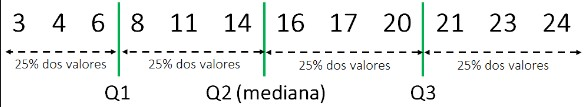
\includegraphics[scale=0.6]{Figuras/slide01_04.jpg}
    \end{figure}
\end{itemize}


\end{ftst}

%=====

\begin{ftst}{Exploração de dados}{Dados univariados}
Uma técnica para visualizar os quartis, mediana e \textit{outliers} é o \textit{boxplots}.
\vone
\begin{figure}
    \centering
    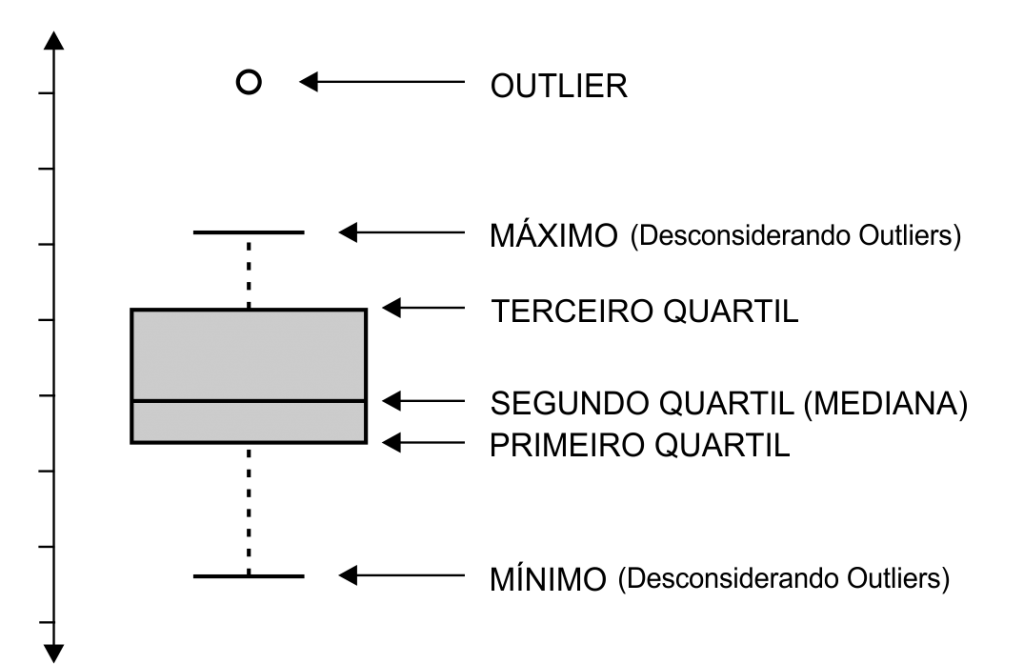
\includegraphics[scale=0.2]{Figuras/slide01_05.png}

\end{figure}


\end{ftst}

%=====

\begin{ftst}{Exploração de dados}{Dados univariados}
\textit{Medidas de espalhamento:} medem a dispersão de um conjunto de valores, permitindo observar se esses estão amplamente espalhados ou relativamente concentrados em torno de um valor. 
\vone
A medidas mais comuns são:
\begin{itemize}
    \item Intervalo.
    \item Variância.
    \item Desvio padrão.
\end{itemize}

\end{ftst}

%=====

\begin{ftst}{Exploração de dados}{Dados univariados}
\small
\textbf{Intervalo:} mostra o espalhamento máximo entre os valores de um conjunto.
\vone
Sejam $x = {x_1, x_2, ..., x_n}$ os valores do atributo para $n$ objetos. O intervalo desse conjunto é medido pela Equação \ref{eq:intervalo}:

\begin{equation}
    \label{eq:intervalo}
    intervalo(x) = \max_{i=1,...,n} (x_i) - \min_{i=1,...,n} (x_i)
\end{equation}

\begin{figure}
    \centering
    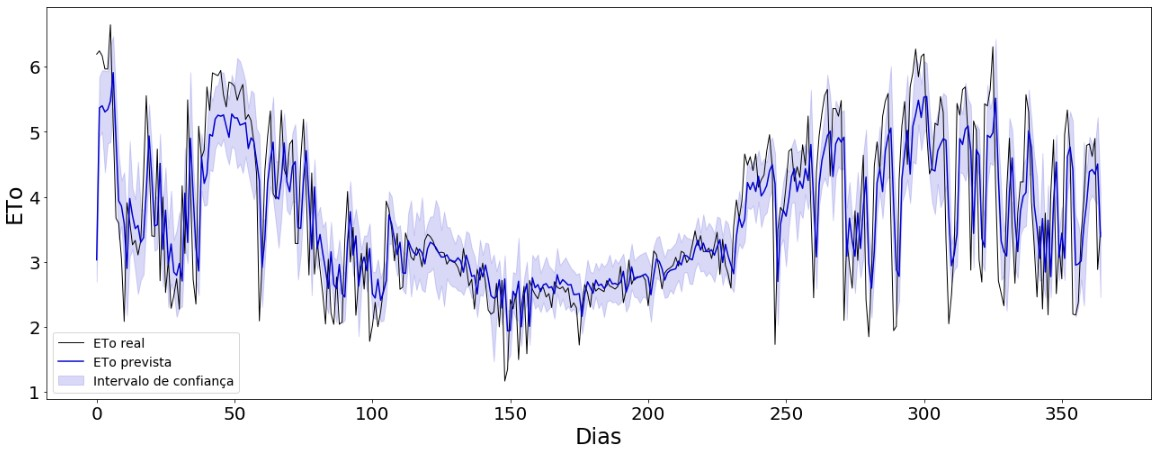
\includegraphics[scale=0.33]{Figuras/ECNN3_interval_2013.jpg}
\end{figure}
\scriptsize
Fonte da imagem: \href{https://bit.ly/2Nvsc0s}{https://bit.ly/2Nvsc0s}
\end{ftst}

%=====

\begin{ftst}{Exploração de dados}{Dados univariados}
\textbf{Variância:} avalia o espalhamento de valores em um conjunto.
\vone
Sejam $x = {x_1, x_2, ..., x_n}$ os valores do atributo para $n$ objetos. A variância desse conjunto é medida pela Equação \ref{eq:variancia}:
\vone
\begin{equation}
    \label{eq:variancia}
    \text{variância}(x) = \frac{1}{n-1} \sum_{i=1}^{n}(x_i - \overline{x})^2
\end{equation}
\vone
Onde: $\overline{x}$ é a média dos valores de $x$.
\vone
Outra medida de espalhamento é o desvio padrão, calculado a partir da raiz quadrada da variância.

\end{ftst}

%=====

\begin{ftst}{Exploração de dados}{Dados univariados}
\footnotesize
\justifying
Para visualizar o desvio padrão e a distribuição dos dados, podemos representá-los em um \textbf{histograma}. Cada barra do histograma possui uma altura proporcional ao número de elementos com aquele valor no conjunto de dados.

\begin{figure}[h]
    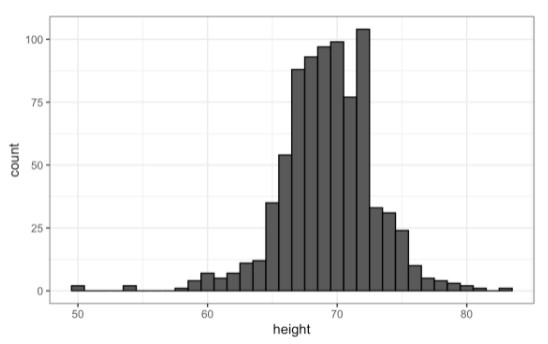
\includegraphics[scale=0.6]{Figuras/histogram.jpg}
\end{figure}



\end{ftst}

%=====

\begin{ftst}{Exploração de dados}{Dados univariados}
\vone
\begin{figure}[h]
    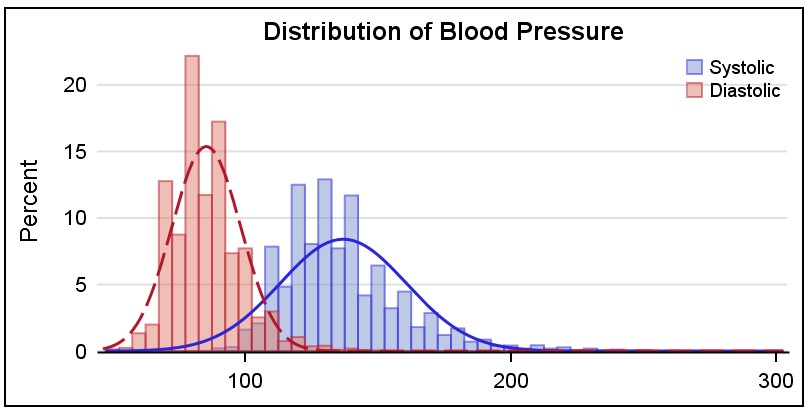
\includegraphics[scale=0.4]{Figuras/slide01_07.jpg}
\end{figure}
\vone
\vone
\vone
\vone
\vone
\scriptsize
Fonte da imagem: \href{http://bit.ly/2Q94jg7}{http://bit.ly/2Q94jg7}
\end{ftst}

%=====

\begin{ftst}{Exploração de dados}{Dados multivariados}
\justifying
\textbf{Dados multivariados:} quando o objeto possui mais de um atributo.
\vone
Nesse caso as medidas de localidade e de espalhamento podem ser obtidas calculando a medida para cada atributo separadamente.
\vone
Dados multivariados ainda permitem análises da relação entre dois ou mais atributos através da medida de \textit{correlação}.

\end{ftst}

%=====

\begin{ftst}{Exploração de dados}{Dados multivariados}
\justifying
\textit{Medida de correlação:} apresenta uma indicação da força da relação linear entre dois atributos. 
\vone
A \textit{matriz de correlação} apresenta a correlação entre cada possível par de atributos de um conjunto de dados, onde de cada elemento tem seu valor definido pela Equação \ref{eq:correlacao}:

\begin{equation}
    \centering
    \text{correlação}(x^i,x^j) = \frac{\text{covariância}(x^i,x^j)}{s_i s_j}
    \label{eq:correlacao}
\end{equation}
\scriptsize
Onde: $x^i$ é o i-ésimo atributo e $s_i$ é o desvio padrão dos valores desse atributo.
\vone
\small
- A correlação$(x^i,x^i) = 1$.

- Correlação positiva: o aumento do valor $x^i$ é acompanhado pelo aumento de $x^j$ e vice-versa.

-Correlação negativa: a redução do valor $x^i$ é acompanhado pelo aumento de $x^j$ e vice-versa.

\end{ftst}

%=====

\begin{ftst}{Exploração de dados}{Dados multivariados}
Para visualizar a relação entre diferentes atributos, podemos usar um \textit{scatter plot}.
\begin{figure}
    \centering
    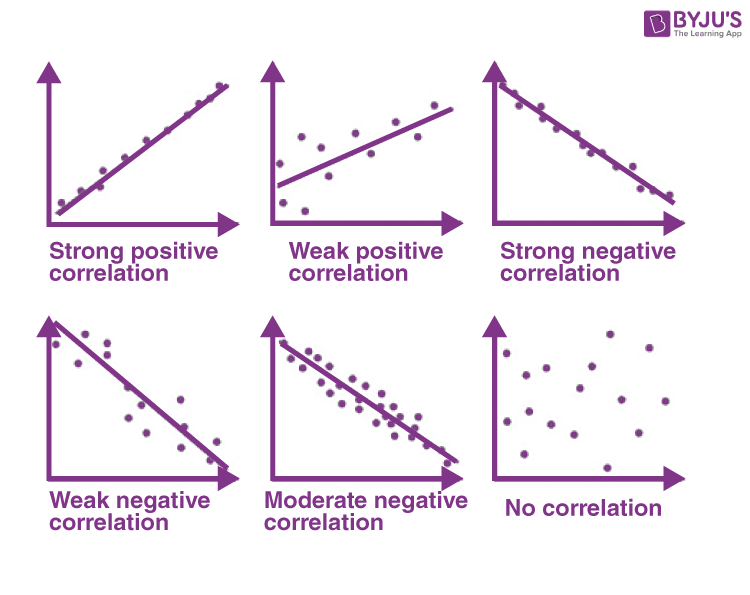
\includegraphics[trim=1cm 1cm 1cm 2cm, clip=true, scale=0.32]{Figuras/slide01_09.png}
\end{figure}
\scriptsize
Fonte da imagem: \href{https://byjus.com/maths/correlation/}{https://byjus.com/maths/correlation/}

\end{ftst}

%=====

\begin{ftst}{Exploração de dados}{Correlação X causalidade}

\begin{figure}
    \centering
    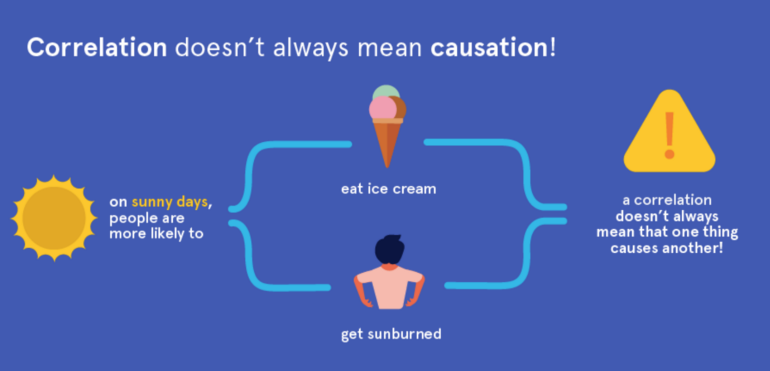
\includegraphics[scale=0.4]{Figuras/slide01_10.png}
\end{figure}
\vone
\vone
\scriptsize
Fonte da imagem: \href{https://medium.com/analytics-vidhya/correlation-causation-977f71bb1e36}{https://medium.com/analytics-vidhya/correlation-causation-977f71bb1e36}

\end{ftst}

%=====


\end{document}